\chapter{Introduction}
\label{chap:introduction}

\textit{There's an infinity of things that have never been done before, and most of those things are not worth doing.} -- Jeremy Fox, \textit{Dynamic Ecology (2016)}~\cite{fox_how_2016}

\begin{center}
\noindent\rule{4cm}{0.1pt}
\end{center}

\selectlanguage{french}
\begin{chapter_summary}{Introduction}
Malgré leur apparente simplicité, les microorganismes sont des êtres vivants complexes capables de survivre dans les milieux les plus extrêmes.
Une telle ubiquité repose en partie sur leurs excellentes capacités d'adaptation.
En effet, \textit{via} l'information stockée dans son ADN, une cellule microbienne est capable, par la production des protéines nécessaires, d'assimiler et de se répliquer à partir d'une grande variété de nutriments.
Ce mécanisme, que l'on appelle l'expression génétique, permet donc à la cellule de réguler sa composition en fonction des conditions environnementales.
Chaque composant cellulaire est initialement issu des ressources trouvées dans l'environnement.
Par l'expression génétique, la machinerie cellulaire résout donc un problème de distribution des ressources: un bien commun (les nutriments) est partagé entre plusieurs milliers de bénéficiaires potentiels (les protéines et autres macromolécules).

Selon quels critères les ressources sont-elles distribuées dans la cellule ?
Le comportement de la plupart des systèmes vivants peut s'expliquer par les principes de la sélection naturelle.
En définissant des facteurs de \textit{fitness} (adaptation au milieu), on peut généralement identifier des objectifs permettant à l'organisme de maximiser sa descendance, et donc de persister sur le long terme dans un milieu donné.
Ces facteurs et surtout leurs importances relatives, peuvent s'avérer extrêmement complexes à identifier, 
ce qui est notamment le cas chez les microorganismes.
Cependant, de nombreuses études ont pu montrer que la maximisation du taux de croissance (ou taux de réplication) est un facteur qui semble commun à de nombreux microorganismes, et qui permet d'expliquer à lui seul une grande variété de comportements.

Peut-on, à l'aide d'un tel principe universel, formaliser la croissance des microorganismes en lois simples, analogues à celle que l'on peut trouver dans d'autres domaines des sciences comme la physique ?
Historiquement, la première tentative d'établissement de lois fondamentales de la physiologie microbienne  fut la découverte de la loi de Monod il y a plus de 60 ans (Fig.~\ref{fig:monod_law} et Eq.~\ref{eq:monod_law}).
Elle montre que le taux de croissance d'un microorganisme suit une loi hyperbolique de la concentration du nutriment limitant dans le milieu.
Depuis, d'autres lois fondamentales ont pu être identifiées.
L'une d'entre elles est une loi de croissance qui décrit la relation linéaire existant entre la concentration en ribosomes dans la cellule et le taux de croissance de l'organisme (Fig.~\ref{fig:scott_rnaprot}).
De manière étonnante, quels que soient les détails moléculaires qui permettent cette adaptation, cette loi émerge lorsque la cellule cherche à maximiser son taux de croissance dans chaque environnement.

Bien que largement répandues, ces lois se limitent cependant à un état bien particulier qu'on appelle croissance à l'état stationnaire.
Cet état est atteint lorsque l'organisme se multiplie pendant suffisamment longtemps dans un environnement stable (Fig.~\ref{fig:growth_curve}).
Il s'avère très pratique pour les études théoriques et expérimentales, notamment car les composants de la cellule ne changent plus au cours de temps, ce qui lui vaut aussi l'appellation de croissance équilibrée (\textit{balanced growth}).
Mais cet état a beau être pratique, il est très loin des conditions rencontrées par les microorganismes dans leur milieu de vie naturel.
Ces derniers sont en effet plutôt soumis à des environnements très changeants, où les éléments chimiques indispensables à la croissance sont rares, et sont donc les objets d'une rude compétition.
Pour quelles raisons les microorganismes seraient-ils optimisés pour un état de croissance qu'ils n'ont quasiment jamais rencontré au cours de leur évolution ?
Si comme on s'y attend ces systèmes sont plutôt adaptés à des environnements variables, ratons-nous quelque chose en ne les étudiant qu'en conditions stables ?

Dans cette thèse, nous nous proposons ainsi d'étendre les études des lois de croissance en adoptant une perspective dynamique, c'est-à-dire, en environnements variables : quelles stratégies dynamiques les microorganismes suivent-ils pour redistribuer leurs ressources lors d'un changement environnemental ?
Cette question sera développée en deux grands axes d'étude.

Quelles sont les meilleures stratégies de distribution des ressources si, comme pour les lois de croissance à l'état stationnaire, la production de biomasse est le seul critère optimisé par la cellule ?
Répondre à cette question est une étape nécessaire pour évaluer dans quelles mesures les critères d'optimisation dynamique peuvent différer de ceux à l'état stationnaire, et donc, de tester si les pressions évolutives s'appliquent effectivement différemment entre environnements stables et dynamiques.
Cette preuve de concept reposera sur un modèle de la distribution des ressources dans une cellule microbienne, qui sera utilisé pour déterminer quelle est la manière dynamique optimale pour la cellule de distribuer ses ressources lors d'un changement d'environnement (Chapitre~\ref{chap:theory}).

Pour tester les prédictions faites expérimentalement, nous chercherons à mesurer cette distribution des ressources chez \textit{Escherichia coli} lors d'une transition de croissance (Chapitre~\ref{chap:experiments}).
Nous montrerons comment l'utilisation de marqueurs fluorescents des ribosomes, d'un dispositif microfluidique de culture continue, et de méthodes originales d'analyse des séries temporelles, permet d'observer et de reconstruire dans le temps l'allocation des ressources lors d'une transition brutale du milieu, notamment la transition d'un milieu pauvre vers un milieu riche (\textit{nutrient upshift}).
\end{chapter_summary}
\selectlanguage{english}

\begin{center}
\noindent\rule{4cm}{0.1pt}
\end{center}

\section*{Beginning of Chapter \thechapter}
\section{Context}
\label{sec:context}

\subsection{Self-replication is a resource allocation problem}

At every moment of our lives, we are surrounded by billions of microscopic organisms.
They sustain themselves by harvesting energy from their environment in the form of organic matter, highly reactive chemicals, or light~\cite{madigan_biology_2006,schaechter_microbe_2006}.
While most of our cells are kept in a stable and friendly internal environment (temperature, oxygenation, nutrient abundance, ...), microorganisms have evolved to constantly adapt their physiology to strongly variable conditions~\cite{mcarthur_microbial_2006,menge_nitrogen_2012,hobbie_microbes_2013,
savageau_escherichia_1983,savageau_demand_1998,blount_unexhausted_2015,vanelsas_survival_2011}.
Not without success, because microbes have been found to survive almost everywhere, sometimes in the strangest places that were initially thought unsuitable for life~\cite{rothschild_life_2001,nicholson_transcriptomic_2012,madigan_biology_2006,schaechter_microbe_2006}.
Such ubiquity translates a strong potential for adaptation.
The model organism \textit{Escherichia coli}, a bacterium first isolated from our intestinal tract, is capable of growing on dozens of different carbon sources through changes in the expression of thousands of genes~\cite{zimmer_microcosm:_2009}.

Microorganisms, along with all living cells, are mainly constituted of polymers (DNA, RNA, proteins) consisting of many repeated subunits (nucleotides, amino acids).
The information about their sequences is stored in the form of genes, physically located on the DNA.
Gene expression is the process by which this information is used in the synthesis of a functional final product (protein or RNA).
The gene expression machinery (itself constituted of RNA and proteins) synthesizes gene products after binding to target sequences either by transcription (promoter on the DNA), or translation (ribosome binding site on the messaging RNA).
In a given cell, there are roughly as many different target sequences as genes~\cite{keseler_ecocyc_2013}, which ensures that not all products are synthesized at the same rate.
Furthermore, some of these products specifically bind some promoters and stimulate or repress promoter activity and hence gene expression.
These products are called transcription factors and allow, in addition to other mechanisms, the regulation of cell composition.

The reorganization of gene expression controls the abundance of enzymes and ribozymes that catalyze the biochemical reactions allowing the cell to perform different functions.
For instance, assimilating a given nutrient involves the synthesis of the corresponding uptake protein and of the metabolic enzymes converting the nutrients into reducing power, nucleotides and amino acids~\cite{schaechter_microbe_2006}.
These precursors are then used to produce new macromolecules, closing the loop of self-replication.
In order to optimize the overall process in different environmental conditions, the cell must adjust the abundance of every enzyme involved in this network of biochemical reactions.
By doing so, the cell actually solves a resource allocation problem, where a common wealth (precursors) has to be distributed over thousands of potential beneficiaries (proteins and other macromolecules).

\subsection{Optimizing biomass production yields a competitive advantage}

Which allocation of resources is optimal for a living cell?
Systems capable of Darwinian evolution sustain themselves in the long run by fitting to their environment~\cite{dawkins_selfish_1976}.
Living cells with the best fitness are more likely to survive, replicate, and through long-term competition, eliminate their siblings.
The optimization criteria that quantitatively measure fitness are called fitness factors.
Whether they apply at the species, the population, the organism, or even the gene level has long been debated~\cite{dawkins_selfish_1976}.
An optimal resource allocation would be a gene expression scheme maximizing the fitness factors.
But since fitness factors have to take into account the ability to survive, reproduce, and compete with other organisms in a given (sometimes changing) environment, they are often context-dependent and highly difficult to identify.

For this reason, there is no consensus about what constitutes the main fitness factors of microorganisms.
Competition for common resources seems to favor the maximization of offspring, in the sense that a replicator with more descendants will outnumber its competitors in the long term~\cite{dawkins_selfish_1976}.
It is unclear, however, how this general principle translates into specific features of microbial physiology.
For instance, the use of genome-scale metabolic network models has shown that metabolism maximizes the production either of biomass or available energy (ATP) depending on the environmental conditions~\cite{schuetz_systematic_2007}.
Microbes can also either optimize their production yield (making the most of available nutrients at the expense of a lower growth rate) or their production rate (growing quickly while wasting part of the available nutrients), the latter being favored in fluctuating environments~\cite{frank_tradeoff_2010,maclean_tragedy_2008,schuster_maximization_2008}.
Overall, it seems that cell optimality drifts in a multidimensional space and involves making several trade-offs that strongly depend on the environmental context~\cite{schuetz_multidimensional_2012}.

Nevertheless, numerous studies have shown that considering growth rate maximization confers a good predictive power of microorganism physiology.
When cultivated in minimal medium with acetate or succinate, \textit{Escherichia coli} uptake rates are correctly predicted by assuming that the metabolic network operates in a mode that maximizes growth rate~\cite{edwards_silico_2001}.
This result is not general though and depends on the carbon source and strain used~\cite{ibarra_escherichia_2002}.
But even in other situations, the metabolic networks evolve rapidly towards growth-rate maximization if a constant nutrient-providing environment is maintained~\cite{ibarra_escherichia_2002}.
The mutants obtained present modications in the regulation of the synthesis of metabolic enzymes~\cite{lewis_omic_2010}, indicating that not only the efficiency of the enzymes is affected, but also their abundance and thus the cellular composition.
Overall, with the currently available knowledge and its limitations (discussed in Chapter~\ref{chap:discussion}), focusing on growth-rate maximization sounds like a rational choice to understand the growth strategies of microorganisms~\cite{molenaar_shifts_2009}.

\subsection{Growth laws are universal strategies employed by microorganisms}

One of the first attempt to formalize the functioning of microbial physiology into elegant, fundamental laws was the discovery of Monod's law more than sixty years ago~\cite{monod_growth_1949}.
This empirical relationship states that the growth rate $\mu$ [\texttt{div~h\textsuperscript{-1}}] of \textit{Escherichia coli} is a hyperbolic function of the concentration of the limiting nutrient $C$ [\texttt{mol~L\textsuperscript{-1}}], such that
\begin{equation}
\label{eq:monod_law}
\mu = \mu_K \frac{C}{K_C + C},
\end{equation}
with $\mu_K$ and $K_C$ two constants depending on the quality of the nutrient (Fig.~\ref{fig:monod_law}).
It is remarkable that the growth rate, a parameter that depends on the use and production of thousands of proteins, can be so easily predicted by a simple relation.
What is even more remarkable is that this relation is rather universal.
Despite some adjustments (the Droop model being a well-known example~\cite{droop_thoughts_1973}), the relation holds for most microorganisms: the growth rate increases with the abundance of the limiting nutrient, up to a point beyond which they cannot grow any faster~\cite{koch_why_1988}.

\begin{figure}[tb]
\centering

\includegraphics[height=5cm]{./Fig/Chapter1/monod_law}
\caption{
\textbf{Monod law, reproduced from~\cite{monod_growth_1949}.}
Monod has been a pioneer in the formalization of microbial growth into fundamental, coarse-grained relationships.
This figure displays the steady-state growth rate (in number of divisions per hour) of \textit{Escherichia coli} in a synthetic minimal medium at 37$^{\circ}$C containing different concentrations of glucose (a common carbon source).
As the concentration of glucose increases, so does the growth rate of \textit{E.~coli} by following the hyperbolic relationship described in Eq.~\ref{eq:monod_law}.
The solid curve is obtained for $\mu_K = 1.35$ div h\textsuperscript{-1}, and $K_C = 0.22 \cdot 10^{-4}$ mol L\textsuperscript{-1}.
}
\label{fig:monod_law}
\end{figure}

The production of every component of the cell is controlled by a complex network of regulatory interactions.
But an obvious constraint is that at steady state, the synthesis rate of all individual components must be proportional to the growth rate in order to compensate for growth dilution~\cite{monod_growth_1949}.
Many physiological parameters (like the mass of DNA, RNA and protein) are thus functions of the growth rate alone, regardless of the environmental conditions~\cite{schaechter_dependency_1958,bremer_modulation_1996}.
These so-called growth laws were carefully measured~\cite{bremer_modulation_1996} and are still used today in the quantitative understanding of growth control in microorganisms~\cite{ehrenberg_mediumdependent_2012}.
Recently, the topic was revitalized through the work of Scott \textit{et al.}~\cite{scott_bacterial_2011}.
They focused on the ribosome concentration, a physiological parameter that was long known to vary linearly with the growth rate in microorganisms (Fig~\ref{fig:scott_rnaprot}).
By measuring it under different environmental perturbations of the protein synthesis machinery, they built a coarse-grained model describing proteome resource allocation~\cite{scott_emergence_2014}.
It has allowed to show that, whatever the details of the molecular implementation (differing between organisms), this growth law emerges from the underlying principles of robustness and optimization imposed by natural selection, especially growth-rate maximization, in all conditions~\cite{scott_emergence_2014}.

\begin{figure}[tb]
\centering
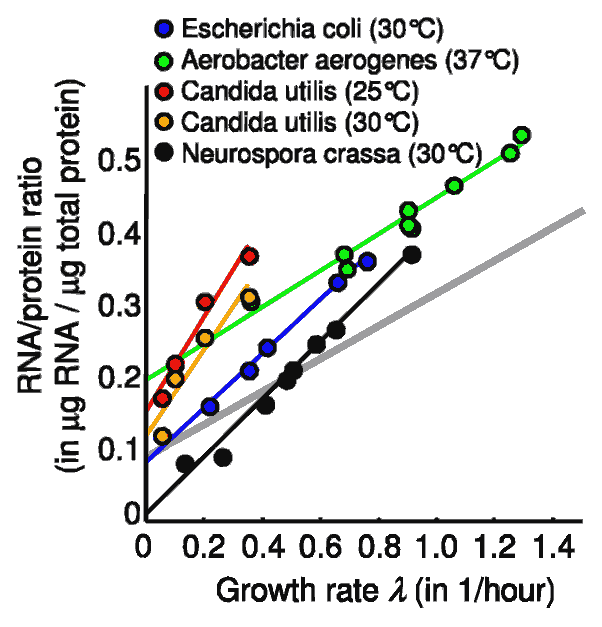
\includegraphics[height=7cm]{./Fig/Chapter1/scott_rnaprot}
\caption{
\textbf{The growth law of ribosomal abundance (figure reproduced from Fig~S1 in~\cite{scott_interdependence_2010}).}
For a variety of carbon sources and their corresponding steady-state growth rate, the RNA/protein ratio is linearly correlated with the growth rate, a relation that holds for many species of microorganisms.
This ratio is correlated with the fraction of ribosome-affiliated proteins, and therefore with the relative abundance of ribosomes in the cell.
}
\label{fig:scott_rnaprot}
\end{figure}

\subsection{Static versus dynamical perspective on growth}

The growth laws cited above apply at steady state, where all intensive properties of the cell are time-invariant~\cite{schaechter_microbe_2006,fishov_microbial_1995}.
This means that the properties that are independent of the cell volume or the cell mass (temperature, concentrations, ...) are constant over time, even though the cell is growing.
It requires that the components of the cell "increase by the same factor over a time interval", which has motivated the use of the term balanced growth~\cite{campbell_synchronization_1957}.
Experimentally, this growth scenario has been used as a standard because it improves reproducibility, in that the results do no longer depend on the precise timing of the samples~\cite{schaechter_microbe_2006}.
It can be easily achieved in the laboratory either in continuous culture, where the substrate is continually supplied~\cite{borirak_molecular_2014}, or in batch conditions if the substrate is in high excess (Fig~\ref{fig:growth_curve}).
This approach has been beneficial to mathematical modeling because considering the system at steady state reduces the complexity of the underlying dynamical system governing microbial growth, allowing genome-scale models encapsulating the enzymatic diversity of living cells to be built and analyzed~\cite{orth_what_2010}.

\begin{figure}[p]
\centering
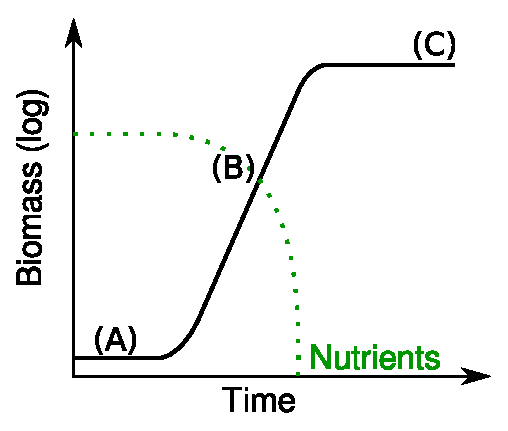
\includegraphics[height=6cm]{./Fig/Chapter1/growth_curve}
\caption{
\textbf{The different phases of a typical growth curve}.
During a typical batch growth scenario, biomass accumulates (black thick line) whereas nutrients are consumed until depletion (green dashed line)~\cite{schaechter_microbe_2006}.
(A) The lag phase is a variable period of time during which the organism adapt to the new medium~\cite{swinnen_predictive_2004}.
It is hard to study experimentaly and is known to be affected by the pre-culturing history of the strain~\cite{ng_damage_1962,dufrenne_effect_1997,shaw_effect_1967}, the magnitude and the rate of the change between the past and present environments~\cite{mcmeekin_predictive_2002}, and other hard-to-control environmental conditions~\cite{cheroutre-vialette_application_2002}.
(B) The steady-state (or balanced-growth) phase is characterized by an exponential production of biomass.
Its characteristics are time-invariant and quite robust accross conditions, which has made it a standard for microbial growth studies~\cite{schaechter_microbe_2006}.
This phase can be extended for hundreds of generations in continuous cultures by the constant renewal of the medium~\cite{borirak_molecular_2014,herbert_continuous_1956,wang_robust_2010}.
As represented here, nutrients are quickly depleted in batch conditions, which does not allow to maintain steady-state growth for a long period of time.
(C) The stationary phase occurs after the depletion of the limiting nutrients in the medium~\cite{chubukov_environmental_2014,schaechter_microbe_2006}.
In natural conditions, microorganisms usually encounter poor media and spend most of their time in stationary phase~\cite{mcarthur_microbial_2006,menge_nitrogen_2012,hobbie_microbes_2013}.
Some species that have evolved long-term resistance mechanisms, like sporulation~\cite{stragier_molecular_1996} or cannibalism~\cite{gonzalez-pastor_cannibalism:_2011}, can survive particularly long stationary phases.
}
\label{fig:growth_curve}
\end{figure}

Although balanced growth is convenient from an experimental and theoretical point of view, it is widely admitted that microorganisms rarely encounter this state in nature~\cite{schaechter_microbe_2006}.
Steady-state growth requires stable conditions over a long period of time, but microorganisms live in
environments where the key elements, such as carbon, nitrogen or phosphorus, are quickly depleted by the competitors as soon as they become available~\cite{mcarthur_microbial_2006,menge_nitrogen_2012,hobbie_microbes_2013}, a consideration that also holds for the lab strains for which growth laws have been established~\cite{savageau_escherichia_1983,savageau_demand_1998,blount_unexhausted_2015,vanelsas_survival_2011}.
Why would microorganisms be optimal for a state they have barely encountered during their evolution?
Are we missing something by studying in stable, unchanging conditions systems that were in fact selected to cope with environmental variations?

\section{Problem statement}
\label{sec:problemstatement}

Microbial growth is essentially a resource allocation problem that can be summarized in simple, fundamental growth laws.
Though established empirically, those laws are elegantly explained if we consider that microorganisms behave in ways that optimize biomass production.
However, these laws describe growth in stable environments and it is hard to imagine how natural selection could have resulted in microorganisms that are optimal for conditions they rarely encounter outside the laboratory.
This motivates the study of growth laws from a dynamical perspective, that is, in a changing environment, and leads us to the following problem statement: \textbf{Which strategies do microorganisms follow in order to dynamically reallocate their resources after a change in the environment?}
The development of this question prompts the following investigations.

What are the best strategies of resource allocation if, like for the steady-state growth laws, we continue to assume that biomass production is the only optimization criterion?
An answer to this question would allow us to assess to which extent the features of dynamical optimization differ from those of steady-state optimization.
In other words, it would test our verbal hypothesis that motivated a dynamical perspective on growth: the expectation that evolutionary pressure applies differently in a changing or stable environment.
In order to achieve this, we need to formulate our problem in mathematical terms, through the development of a proof-of-concept model of resource allocation in bacterial cells, and the theoretical determination of the optimal dynamical allocation of resources following a change in the environment.

The model will help us to establish actual resource allocation strategies that optimize biomass production during an environmental change.
However, it will not be able to tell us if microorganism do actually optimize such a criterion.
We therefore need to measure biomass accumulation and changes in resource allocation following a change in the environment.
How could one measure resource allocation during a growth transition?
In the light of the discussion in the previous section, this requires monitoring the abundance of key macromolecules in living cells over time, while establishing an experimental set-up that allows to control the inherent variability of dynamical experimental studies of microbial growth.

\section{Related work}

\subsection{Modeling growth of microorganisms}

My recent experience as a teacher taught me that, as of today, many students in biology do not like mathematics very much.
Since mathematics is the main language of modeling, this has often made it difficult for me to convince them that modeling is of key importance for biologists.
However, while mathematics is the language, it is not the essence of modeling.
Generally speaking, a model depicts and simplifies reality.
Maps, sketches, or pictures satisfy this definition, as do graphs, sets of equations, or even the DNA sequences stored in a text file on a computer.
In other words, depicting and simplifying reality makes you a modeler, not so much drawing equations on a board.
But this does not change the fact that mathematics are powerful tools for formulating and analyzing models~\cite{servedio_not_2014,mcgill_calm_2013}.

What makes mathematical modeling so useful in microbial growth studies?
%Evolutionary biology is a good example of a field that has relied on mathematical modeling for a long time~\cite{servedio_not_2014}.
%The large time and population scales at which evolutionary processes occur complicate experimental work, despite several attempts on organisms with a short generation time~\cite{barrick_genome_2013,elena_evolution_2003,kassen_experimental_2002,schneider_dynamics_2004}.
%Besides, microbiology is a field particularly prone to experimental study.
%A growth curve as presented in Fig.~\ref{fig:growth_curve} can be made in a day, so the limitations of evolutionary biology should not apply to microbial growth studies.
%But as knowledge and experimental data on microbes accumulates, the need for a systemic understanding of biology is more and more pressing~\cite{alon_introduction_2006,kremling_systems_2013,hillis_why_1993}.
Microbial physiology results from the interplay of thousands of chemical reactions that are not necessarily relevant in any given situation~\cite{schaechter_microbe_2006}.
These reactions occurs on a wide range of time scales (shorter than 1~second for metabolism, to more than 1~day for the degradation of stable proteins~\cite{schaechter_microbe_2006}), and are controlled by several layers of regulatory mechanisms that can only be understood through evolutionary considerations~\cite{dawkins_selfish_1976}.
As a consequence, even the simplest verbal hypothesis can resist direct empirical testing.
But abstracting away complexity is the purpose of mathematical models.
The overwhelming number of variables and the co-existence of several different time scales can be dealt with by choosing the correct framework.
When working on a model, microbial behavior is abstracted into a world of clearly stated rules, where it is easier to spell out the logical consequences of the underlying assumptions~\cite{servedio_not_2014,mcgill_calm_2013}.
Predictions can be made, "unpacked" into our real world, and confronted with experimental testing.

Modeling has proven to be particularly helpful in unveiling how metabolic networks operate.
For an increasing number of microorganisms, we are now able to draw quasi-exhaustive maps of their metabolic reactions.
For instance, a much-used genome-scale reconstruction of \textit{E. coli} metabolism contains 1366 genes, 2251 metabolic reactions, and 1136 unique metabolites~\cite{orth_comprehensive_2011}.
The number of variables may seem overwhelming, and making sense of this information is not straightforward.
Which reactions are important, and in which environmental conditions?
Can we predict how perturbations will affect a given metabolic network?
Do fundamental regularities exist between different metabolic networks, from different species?

The complexity of the reconstructed metabolic networks does not impede their mathematical study.
Constraint-based modeling is a framework that abstracts away the unknown kinetics and represents the metabolic reactions by steady-state fluxes to which physico-chemical constraints can be applied, e.g., compartmentalization, mass conservation, molecular crowding, and thermodynamic directionality~\cite{ebrahim_cobrapy_2013}.
From a mathematical point of view, the model consists of a system of linear equations defining a space of admissible flux distributions that is further reduced by the above-mentioned constraints, which eliminate flux distributions that are unlikely to occur in an environmental condition of interest.
The solution space is often further reduced by selecting the flux distributions optimizing a specified objective function, such as the growth rate of the cell.
This approach, called flux balance analysis (FBA)~\cite{orth_comprehensive_2011,palsson_systems_2011}, has been shown to correctly predict many behaviors of the metabolic network of \textit{E. coli}~\cite{varma_stoichiometric_1994,edwards_silico_2001}.
It has also proved capable of predicting its long-term adaptation through evolution of the network after a gene deletion~\cite{fong_metabolic_2004}.

More direct modeling approaches, in the form of large kinetic models, have also been helpful for understanding growth-related processes.
Through the construction of a model of 47 differential equations and 193 parameters, Kotte \textit{et al.} have shown how metabolic fluxes are sensed at different locations in central carbon metabolism, and are integrated in a global cellular response by the coupling of enzymatic and transcriptional regulation~\cite{kotte_bacterial_2010}.
Kinetic models of this type are sufficiently detailed to be used as an \textit{in silico} testbed to investigate specific molecular mechanisms and uncover their function in bringing about a cellular response~\cite{peskov_kinetic_2012}.
The most emblematic instance of this approach is probably the recent whole-cell model of \textit{Mycoplasma genitalium}~\cite{karr_whole-cell_2012}.
By aggregating all the available knowledge from more than 900 publications, Karr \textit{et al.} constructed a dynamical model accounting for all the annotated gene functions of this pathogenic organism, and successfully used it to investigate unobserved molecular mechanisms and guide novel experimental analysis.
While such approach is not yet applicable to many organisms, it genuinely demonstrates how the increase in computational power could one day guide \textit{in silico} experimentation.

The granularity of the kinetic models cited above is their strength, but also their main weakness.
Despite the available knowledge of molecular mechanisms, precisely measuring \textit{in-vivo} kinetic parameters still represents a technological bottleneck~\cite{park_metabolite_2016,bennett_absolute_2009,buscher_cross-platform_2009}.
While parameter values can be collectively fitted to available data~\cite{jaqaman_linking_2006,mendes_non-linear_1998}, this is known to often produce large parameter uncertainty~\cite{cho_experimental_2003,brodersen_characterization_1987,rodriguez-fernandez_hybrid_2006}.
This is problematic, because the predictions are often particularly sensitive to the parameter values~\cite{gutenkunst_universally_2007,ingram_network_2006,mayo_plasticity_2006}.
Constraint-based modeling overcomes this limitation by using a mathematical approach that does not require any knowledge about the reaction kinetics.
The drawback is that this approach strongly depends on the constraints used to reduce the space of admissible solutions, e.g. the choice of the objective function that may be tricky, as discussed above~\cite{kauffman_advances_2003}.

The limitations of constraint-based and detailed kinetic models have motivated the construction of simpler, coarse-grained models.
The philosophy is quite different: instead of aggregating all available knowledge into a detailed model, the modeler is concerned about carefully filtering this information to keep the model as simple as possible.
The resulting models generally describe cellular functioning on a high level of abstraction, and are particularly valuable when looking for universal laws or principles~\cite{scott_bacterial_2011,scott_interdependence_2010,scott_emergence_2014}.
They can take the form of minimal core models that focus on a given aspect of growth, while still abstracting away the molecular details (see \textit{e.g.}, ~\cite{spiesser_size_2012}).
They can also be used as proof-of-concepts to submit verbal hypotheses to the logic and rigor of mathematical reasoning~\cite{servedio_not_2014}.
For instance, a simple proof-of-concept model was used to uncover the principles leading to overflow metabolism, a mechanism by which microorganisms switch to inefficient metabolic pathways when growing at high nutrient availability~\cite{molenaar_shifts_2009}.
This paradoxical and widespread phenomenon~\cite{dijken_kinetics_1993,vemuri_overflow_2006,mckeehan_glycolysis_1982,hsu_cancer_2008} was shown to be easily explained by the fact that high yield pathways also require the synthesis of more enzymes, revealing the occurrence of a cost-benefit trade-off producing the switch when nutrients are no longer the limiting factor.
Overall, these models have several advantages for the purpose of our study: they clearly state the underlying assumptions, and are sufficiently tractable to be analyzed by a variety of mathematical tools.

%It is also the preferred approach when one wants to broaden its access to mathematical tools~\cite{vandenberg_optimal_1998}, most of them being unhelpful with the high dimensionality of biological models.
%As we will describe in section~\ref{sec:approach}, this represents the modeling strategy that was used in this thesis.

%\begin{figure}[tb]
%\centering
%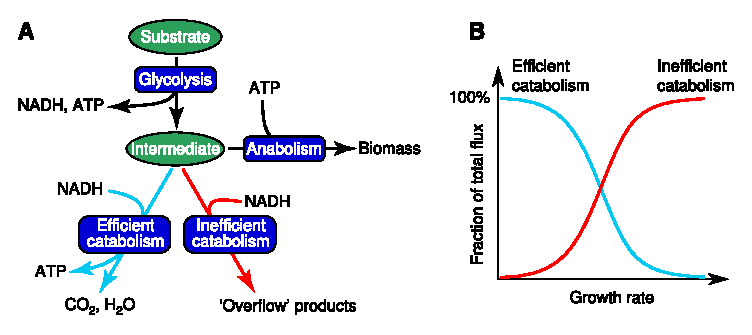
\includegraphics[width=\textwidth]{./Fig/Chapter1/molenaar_overflow.eps}
%\caption{
%\textbf{The strategy of overflow metabolism, reproduced from~\cite{molenaar_shifts_2009}.}
%When increasing the concentration of substrate, the metabolism of microorganisms switches toward the use of inefficient pathways.
%This paradoxical behavior does in fact maximize the growth rate if we take into account the costs and benefits of enzyme synthesis, in particular the fact that pathways for inefficient catabolism are shorter and therefore cheaper to produce.
%(A) Simple view of microbial metabolism, with the two competing efficient and inefficient pathways.
%(B) The switching from efficient to inefficient catabolism when the concentration of nutrients, and hence the growth rate, increases.
%}
%\label{fig:molenaar_overflow}
%\end{figure}

\subsection{Measuring growth of microorganisms}

Either to formulate hypotheses or test predictions, data on microbial growth need to be acquired.
The most straightforward method is to work at the population level.
When working with microorganisms, a clonal population of genetically identical cells can easily be obtained by inoculating a single colony into a growth medium~\cite{schaechter_microbe_2006}.
Over time, this culture can be subjected to different types of measurements: for instance, biomass can be estimated  directly through measurements of the dry weight of samples~\cite{monod_growth_1949}, or indirectly through measurements of transmitted or scattered light across the culture~\cite{volkmer_condition-dependent_2011}, allowing to construct growth curves as presented in Fig.~\ref{fig:growth_curve}.
Other population-wide parameters, like the macromolecular composition~\cite{scott_interdependence_2010,scott_bacterial_2011} or the concentration of metabolites~\cite{bennett_absolute_2009} can also be evaluated.
They represent averaged estimates from billions of genetically identical cells and are thus usually robust and reliable measurements.
In fact, most of \textit{E.~coli} parameters that are currently used in today's growth models have been measured at the population level, notably through the emblematic work of Bremer and Dennis~\cite{churchward_macromolecular_1982,bremer_modulation_1996,bremer_free_2003,bremer_feedback_2008}.

Nevertheless, some questions cannot be solved at the population level~\cite{davey_flow_1996,bakshi_superresolution_2012,balaban_bacterial_2004}.
One example are questions about the internal structure of the cell~\cite{bakshi_superresolution_2012}.
Bakshi \textit{et al.} used a combination of fluorescent labeling and superresolution imaging to localize the ribosomes, RNA polymerases and DNA in living \textit{E.~coli} cells~\cite{bakshi_superresolution_2012}.
They showed that despite what was previously thought, most of the translation occurs far from the DNA, on free mRNA molecules that migrate to ribosome-rich regions~\cite{bakshi_superresolution_2012}.
Another example concerns questions about single-cell variability~\cite{balaban_bacterial_2004,booth_stress_2002,sumner_phenotypic_2002}.
Through growth and imaging of single cells in a microfluidic device, Balaban \textit{et al.} showed that a clonal bacterial population can profit from a preexisting heterogeneity to persist when challenged by the presence of an antibiotic, a short-term mechanism that does not involve any genetic mutation~\cite{balaban_bacterial_2004}.
In the long term, heterogeneity has also been shown to help subpopulations to resist lethal stresses, leaving them with enough time to adapt and conquer new ecological niches~\cite{booth_stress_2002,sumner_phenotypic_2002}.
In fact, cell heterogeneity seems so crucial for the fitness of microorganisms that diversity-generating mechanisms have been identified~\cite{true_yeast_2000,fraser_noise_2004,raser_control_2004}.

In addition to the level of measurement, the cultivation method plays a significant role in the kinds of question that an experiment can answer.
With the advent of molecular genetics in the 1970s and 1980s, batch growth conditions have been the preferred choice of most microbiologists~\cite{hoskisson_continuous_2005}.
As illustrated in Fig.~\ref{fig:growth_curve}, the organism is inoculated in a closed-system and grows until the nutrient is depleted.
In a sense, such a condition is close to what microbes encounter in nature, where key nutrients are only available for a short time and quickly depleted~\cite{mcarthur_microbial_2006,menge_nitrogen_2012,hobbie_microbes_2013}, and is essential to study many questions, \textit{e.g.} diauxic growth~\cite{kremling_understanding_2015}.
Currently, a strong advantage of batch culturing is the intense parallelization that can be attained using microplates.
Indeed, microplates allow to perform dozens to hundreds of growth experiments, each in less than one milliliter, while the optical density or the fluorescence of each culture is automatically monitored.
This has proven extremely helpful for screening purposes and the establishment of standard libraries of gene labeling and modification~\cite{baba_construction_2006,zaslaver_comprehensive_2006}.
Parallel cultivation has notably been exploited to construct roughly 4,000 single-cell knock-out mutants of \textit{Escherichia coli}, forming the Keio collection~\cite{baba_construction_2006}.
This mutant collection was extensively used during the last decade to unveil unknown gene functions and test genome-wide effects of gene deletions (as of 2009, more than 4~millions samples issued from this collection had been shared worldwide~\cite{yamamoto_update_2009}).
Microplates have also helped building a massive library of transcriptional fusions of the green fluorescent protein to each of about 2,000 different promoters in \textit{E.~coli}~\cite{zaslaver_comprehensive_2006}.
Interestingly, microplate batch growing conditions have also been used when applying the above constructions in the inference and analysis of gene regulatory networks~\cite{gerosa_dissecting_2013,berthoumieux_shared_2013,keren_promoters_2013,
ronen_assigning_2002,stefan_inference_2015}.
But the latter use can be hazardous, because the main drawback of the batch condition is that the culturing system is poorly controlled.
Changes of key chemical parameters (\textit{e.g.} pH, pO\textsubscript{2}) have been shown to occur during the whole growth curve~\cite{bekker_changes_2007}. 
At high density, metabolic by-products can accumulate in the medium and impede growth before nutrients are exhausted~\cite{ackerman_accumulation_1974,lenski_chemical_2002,luli_comparison_1990}.
This could be dealt with by focusing on the beginning of the culture, but this part has been shown to strongly depend on the preculture history~\cite{ng_damage_1962,dufrenne_effect_1997,shaw_effect_1967}, and one is never sure when an internal steady state has been reached~\cite{myers_culture_1944}.
%[NB THE FACT THAT CULTURE CONDITIONS CHANGE IS NOT NECESSARILY "HAZARDOUS", IF ALL MEASUREMENTS USED FOR THE INFERENCE PROCESS HAVE BEEN OBTAINED UNDER THE SAME CONDITIONS. THE CHANGE IN CONDITIONS IS ALSO A PERTURBATION OF THE NETWORK AND POSSIBLY INFORMATIVE...]
% Nils: Indeed, but I need to make a point here in order to motivate why we used complicated culture.

For this reason, continuous cultures were developed for microbial studies~\cite{myers_culture_1944,novick_experiments_1950,herbert_continuous_1956}.
Through the permanent renewal of the growth medium, continuous cultures allow for maintenance of a chemically well-controlled environment, allowing for the acquisition of reproducible and reliable data~\cite{borirak_molecular_2014,hoskisson_continuous_2005}.
This has shown to be particularly valuable for comparative omic analysis, for instance the analysis of changes in protein levels~\cite{kolkman_comparative_2005} or genome-wide transcriptomic changes~\cite{boer_genome-wide_2003} that occur when \textit{Saccharomyces cerevisiae} is grown in different media.
Continuous cultures are more difficult to set-up, however~\cite{novick_experiments_1950,borirak_molecular_2014}.
Even if the working volume can be reduced~\cite{betts_miniature_2006}, they usually consume large quantities of medium and are, by design, expected to be more prone to contamination~\cite{novick_experiments_1950}.
But recent advances in microfluidic technology have made it possible to set up robust continuous cultures experiments on the microliter scale~\cite{wang_robust_2010,balaban_bacterial_2004}.
For instance, the mother machine~\cite{wang_robust_2010} allows to perform long-term growth of microorganisms
in continuous culture using only a few milliliters of fresh medium per hour.
This has enabled to show that \textit{E.~coli} growth is remarkably stable on the long term and rather immune to the aging mechanisms that normally affect mother cells in other microorganisms.
It is however important to note that at those scales, growth can only be monitored through microscopy analysis, which could unnecessarily complicate studies that do not rely on single-cell measurements.

The experimental approaches briefly reviewed above can be applied to study microbial growth in a dynamical setting~\cite{levy_strategy_2007,levy_coordination_2009,madar_promoter_2013,ehrenberg_mediumdependent_2012}.
For instance, Levy \textit{et al.}~\cite{levy_strategy_2007,levy_coordination_2009} applied pulse-like environmental perturbations to a continuous culture of yeast, and measured how transcriptomic reorganization occurs.
They observed that the transcription levels are affected before the growth rate of the organism, suggesting a significant role of feed-forward sensing from the environment.
Madar \textit{et al.}~\cite{madar_promoter_2013} analyzed the transcriptional reorganization occuring in \textit{E.~coli} during the lag phase through the coupling of batch experiments in microplates and single-cell measurements \textit{via} flow cytometry.
They showed that \textit{bottleneck enzymes} were produced early in the lag phase, before the cells actually switch to the production of ribosomes and general metabolic enzymes.
As in this PhD project, the studies cited above investigate questions that can only be answered in a dynamical context and they inspired the search for the most appropriate experimental approaches to answer the problem set out in Section~\ref{sec:problemstatement}.
By taking the best of the works presented above, a part of our study will focus on establishing such experimental conditions.

\section{Approach}
\label{sec:approach}

Throughout this study, we focus on a specific dynamical growth scenario, namely the case of a nutrient upshift~\cite{ehrenberg_mediumdependent_2012,kjeldgaard_kinetics_1961,schaechter_patterns_1961,johnsen_control_1977}.
Contrary to steady-state growth, nutrient upshifts and downshifts are frequently encountered in the life cycle of microorganisms~\cite{schaechter_microbe_2006,mcarthur_microbial_2006,menge_nitrogen_2012,hobbie_microbes_2013}.
In combination, they also provide a good approximation of more complex environments.
In nature, nutrient upshifts generally start from stationary phase~\cite{mcarthur_microbial_2006,menge_nitrogen_2012,hobbie_microbes_2013}, a state in which complex adaptive mechanisms are at work that we would like to sidestep for this study~\cite{stragier_molecular_1996,gonzalez-pastor_cannibalism:_2011,ng_damage_1962,dufrenne_effect_1997,shaw_effect_1967,mcmeekin_predictive_2002,cheroutre-vialette_application_2002}.
For this reason, we confine the problem to the study of resource allocation during a so-called steady-state-to-steady-state transition.
While we expect the starting and ending conditions to be on the growth law presented in Fig.~\ref{fig:scott_rnaprot}, we currently have no idea of what happens in the time between.

We start by developing in Chapter~\ref{chap:theory} a simple proof-of-concept model of resource allocation that evaluates how biomass production can be maximized during an upshift from a medium with low nutrient content to a medium with high nutrient content.
The model is an instance of a self-replicator model~\cite{molenaar_shifts_2009}, but focuses on the allocation of resources to only two sectors of the microbial cell: metabolism, taking up and converting nutrients to precursor metabolites, and gene expression, producing macromolecules from the precursors.
The model is kept as simple as possible in order to make sure it stays mathematically tractable in a dynamical context.
A necessary step is however to verify that, at steady-state, the model account for known growth laws of resource allocation~\cite{scott_interdependence_2010,scott_bacterial_2011}.

Using this model, we pose the problem of dynamical optimization as an optimal control problem~\cite{stengel_optimal_1994}.
To comply with what we know at steady state, the microbial cells are assumed to maximize biomass production, but we adapt the criterion to the dynamical context of an upshift scenario.
By using a combination of analytical~\cite{carlson_infinite_1991} and numerical optimization~\cite{bonnans_bocop_2012}, we aim to identify a mathematical upper bound for the biomass produced~\cite{stengel_optimal_1994}.
This theoretical solution can then be used to explore possible regulatory strategies.
In particular, we use the bang-bang~\cite{stengel_optimal_1994} control solution found as a benchmark to identify the system variables that need to be sensed in order to optimize resource allocation.
This provides a common scale on which the outcomes of different regulatory schemes can be compared during an upshift scenario.
This allows us to identify one or several strategies that clearly outperform all the others, giving us testable predictions.
Specifically, we show that feedback from the intracellular state turns out to be much more valuable than information from the environment.
We investigate if such a strategy could be active in real cells, and identify the widespread ppGpp system~\cite{bosdriesz_how_2015} as a possible molecular implementation that could control the synthesis of ribosomes in a switch-like manner during a nutrient upshift.
Overall, this chapter demonstrates that, if microbial cells actually optimize their biomass production during an upshift, they should dynamically allocate their resources to the gene expression machinery in an on-off manner, making an experimentally testable prediction.

In Chapter~\ref{chap:experiments}, we address the challenging problem of experimentally verifying this prediction in \textit{Escherichia coli}.
This task requires the development of an experimental set-up allowing the measurement of resource allocation in our dynamical growth scenario, \textit{i.e.} a steady-state-to-steady-state nutrient upshift.
From the model developed in Chapter~\ref{chap:theory}, we identified that the predicted on-off pattern should occur on a short time scale after the transition (a couple of generations).
This motivates the use of \textit{in-vivo}, high-frequency, single-cell measurements of the concentration of the gene expression machinery.
Inspired by the work of Bakshi \textit{et al.}~\cite{bakshi_superresolution_2012}, we constructed a strain with a GFP-tagged S2 ribosomal subunit, grew this strain in the mother machine, and monitored expression of the reporter gene using fluorescence microscopy~\cite{wang_robust_2010}.
While originally developed for studies of long-term steady-state growth, we used the mother machine here to perform an instantaneous medium transition in a controlled manner from acetate (a poor carbon source) to glucose (a rich carbon source), in order to obtain a significant difference in growth rates between the two media~\cite{andersen_are_1980}.

After segmentation and cell tracking, this set-up was able to generate fluorescence and size time series for dozens of cells.
Using again the self-replicator model as a framework, we showed that these measurements are sufficient for the intended signal reconstructions, in particular the growth rate and the resource allocation profile over time.
The method we used is called Kalman smoothing~\cite{kailath_linear_2000,jazwinski_stochastic_2007}.
While well-known in engineering, Kalman smoothing has been rarely used in quantitative biology, but turned out to be particularly suitable for the purpose of the model-based analysis of gene expression data in single cells, as we argue and show on synthetic data in Chapter~\ref{chap:experiments}.
Finally, the experimental verification or falsification of the optimal control prediction, should allow to conclude whether the biomass maximization, as considered in Chapter~\ref{chap:theory}, is indeed a cell objective in a dynamical context.